
\documentclass[]{report}
\usepackage{pdfpages} 
\usepackage[utf8]{inputenc}
\usepackage[spanish]{babel}
\usepackage{graphicx}
\usepackage{subfigure} % subfigura
\graphicspath{ {images/} }
\usepackage{afterpage}
\usepackage{cite} % para contraer referencias
%\usepackage{hyperref}
\usepackage{blindtext}
\usepackage[ruled,vlined,linesnumbered]{algorithm2e}
\usepackage{url}
\usepackage{listings}
\usepackage{algpseudocode}
\usepackage{verbatimbox}
\usepackage{amsmath}
\usepackage[Sonny]{fncychap}
%\usepackage[options ]{algorithm2e}
%\usepackage{algorithm}
% Title Page

\title{TESIS}
\author{Efren López Jiménez}


\begin{document}
	
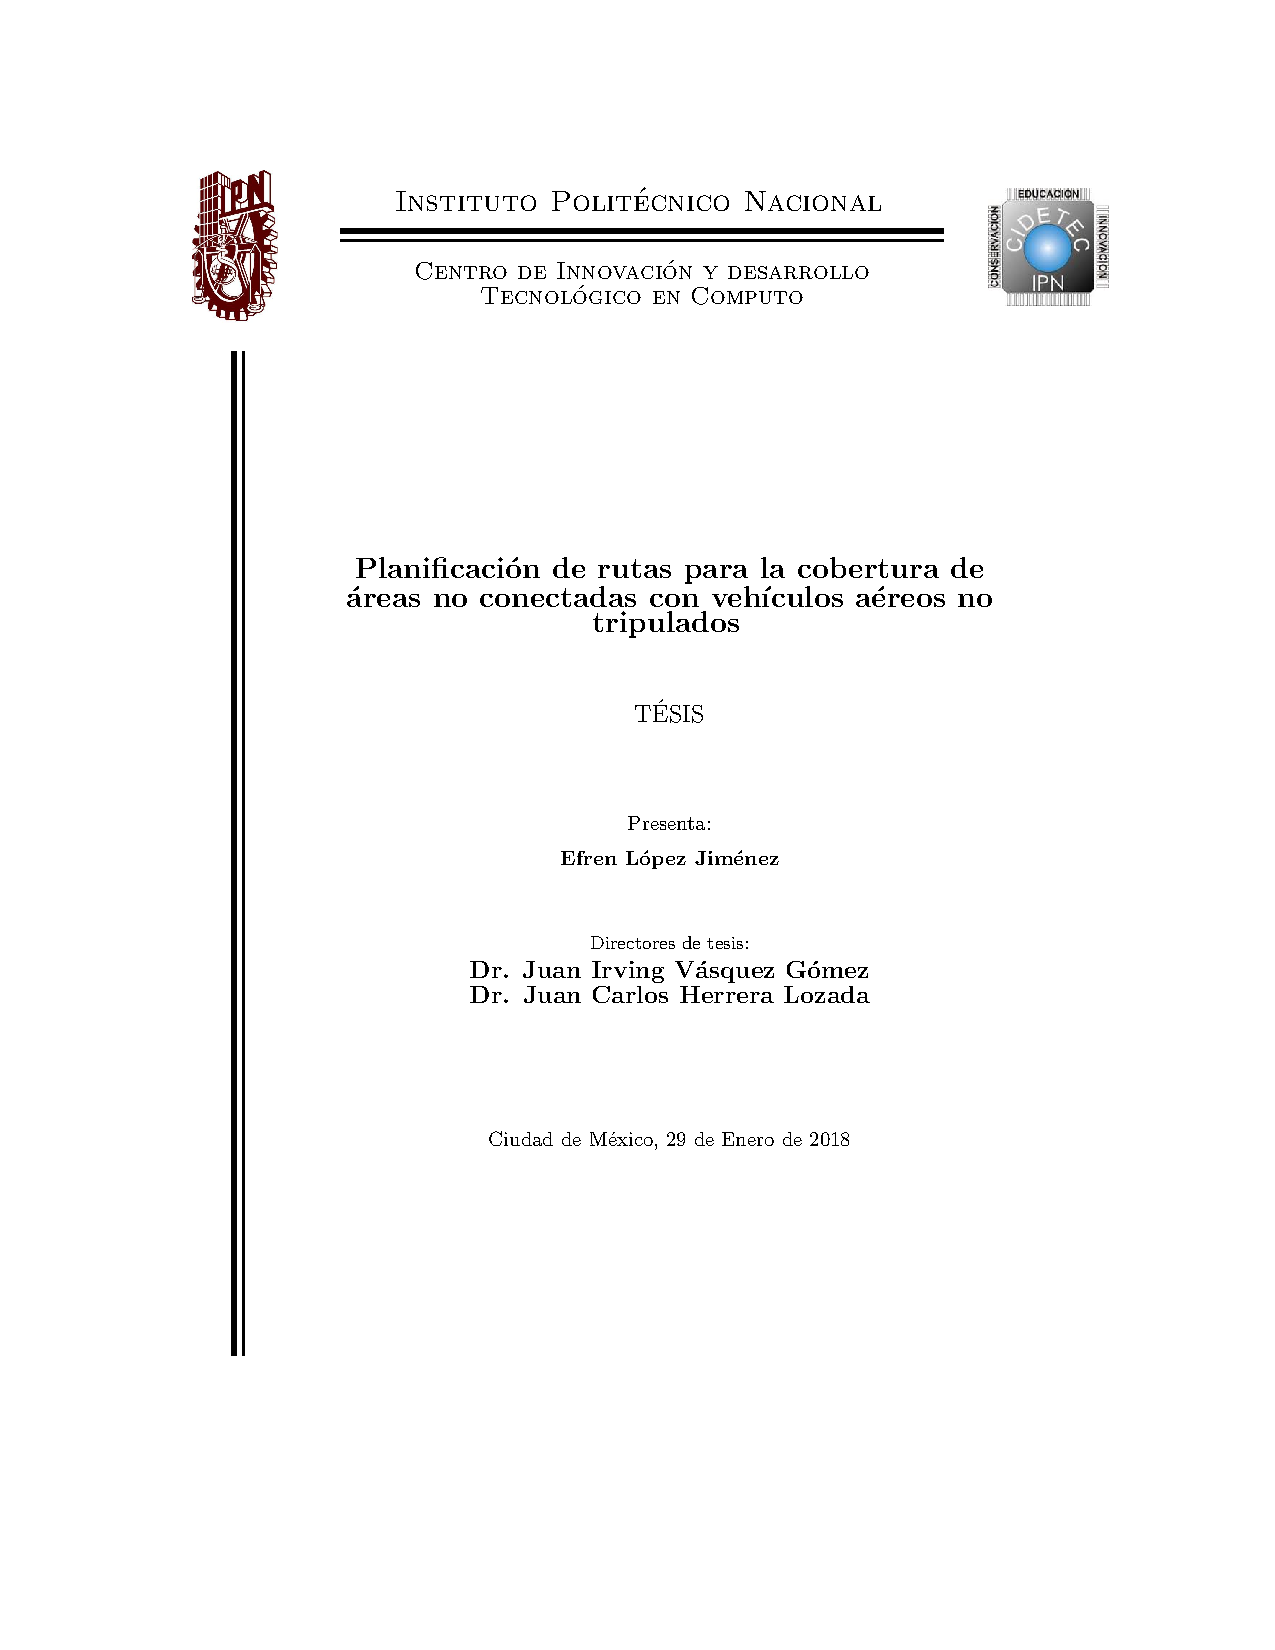
\includepdf[pages={1}]{portada.pdf}
	

\newpage\null\thispagestyle{empty}\newpage
	
%\maketitle

\begin{abstract}
	

\end{abstract}
\afterpage{\null\newpage}
\newpage
\addtocontents{toc}{\hfill \textbf{Página} \par}
\tableofcontents
\listoffigures
\listoftables
\def\BState{\State\hskip-\ALG@thistlm}

\chapter{Introducción}
El uso de vehículos aéreos no tripulados ha trascendido en diferentes tareas de aplicación, en conjunto con otras ramas de la computación es posible aplicar conocimientos de ingeniería, en aplicaciones como agricultura de precisión, mediante el análisis, procesamiento de imágenes, planificación de rutas, es posible monitorear el estado de salud de las plantas, detectar el estado hídrico, el estado nutricional, detección temprana de enfermedades y plagas, entre otros, evaluación de daños y con esos datos sustentar la decisión final para el aprovechamiento adecuado de dichas plantas, en tareas de vigilancia con ayuda de planificación de trayectorias, adquisición-procesamiento de imágenes, facilita la localización especifica del objetivo a perseguir.

La exploración de áreas y terrenos ha sido estudiada varios años atrás, se han probado diferentes maneras de resolver el problema de cobertura de área a su vez utilizando algoritmos que permitan una planificación eficiente para la búsqueda de un objetivo en particular, por ejemplo con móviles terrestres, utilizando diferentes algoritmos, donde tienen un objetivo final, la exploración de un área en particular teniendo aplicaciones en diferentes áreas de investigación, por ejemplo robots contra incendios, robots de rescate, etc.

Un vehículo aéreo no tripulado (VANT) es una aeronave sin tripulación a bordo, con características particulares para realizar vuelos y es controlada remotamente por un piloto mediante un sistema de control.
\\Durante los últimos años la importancia del uso de los VANT, se ha beneficiado el crecimiento y desarrollo de las Tecnologías aéreas en los sectores de producción y servicio con la finalidad de facilitar tareas científicas y cotidianas, gracias a estas tecnologías, la autonomía de dichos móviles aéreos se ve reflejada en disminuir el riesgo la mano del hombre en los procesos peligrosos.
\\Los vehículos aéreos no tripulados o robots aéreos, permiten el desarrollo autónomo o semiautomático de diferentes tipos de misiones que cubren desde los sectores de defensa de seguridad a los de agricultura y medio ambiente.\cite{srBarrientos}\\

La importancia de estudiar los vehículos aéreos, empieza cuando se requiere explorar zonas de alta peligrosidad, o zonas complejas donde implica un riesgo al ser humano.
Uno de los retos a enfrentar en el área de robótica con vehículos no tripulados, es la planificación de rutas no conocidas, que nos permitan conocer o explorar un área independientemente de la utilidad u objetivo que se pretenda realizar. Los experimentos pueden ser con obstáculos complejos o determinar un espacio en particular, la idea se genera a partir de la necesidad de reducir el tiempo de vuelo, cubriendo en su totalidad un área de interés en particular.
Las carga de la batería de los vehículos aéreos tienen un periodo determinado para alimentar al robot, sin embargo, la importancia de considerar este recurso limitado implica delimitar de manera puntual al momento de planificar el vuelo.
\section{Motivación}
La importancia de dotar autonomía a un robot hoy en día es indispensable para realizar actividades en zonas de riesgo para los seres humanos, en el caso de los vehículos aéreos dadas sus limitantes como la duración de las baterías, el poco alcance de los sistemas vía inalambrica para maniobrabilidad y su uso en diferentes aplicaciones científicas y tecnológicas es necesario implementar técnicas que nos permitan realizar una trayectoria óptima aprovechando mejor los recursos que dichos vehículos nos ofrecen.\\
El uso de dichas tecnologías se pueden implementar en los diferentes campos de conocimientos y el área tecnológica, dado que hay infinidad de  problemas de aplicación que se podría resolver con el uso de dichas técnicas computacionales, por ejemplo en la agricultura de precisión para identificar el estado de salud de las plantas, en el área de inspección, entre otros.

%\subsection{Planificación de rutas}

  


\section{Problema}

Debido a la importancia de  obtener información de terrenos  de difícil acceso con un conjunto de características no conocidas {\bfseries ''se tiene la necesidad de cubrir un conjunto de polígonos de forma autónoma mediante un sistema embebido a bordo de en un VANT ''} , minimizando el costo en función de la necesidad de obtener información necesaria para una determinada aplicación (Fig 1.1).
\begin{figure}[!h]
	\centering
	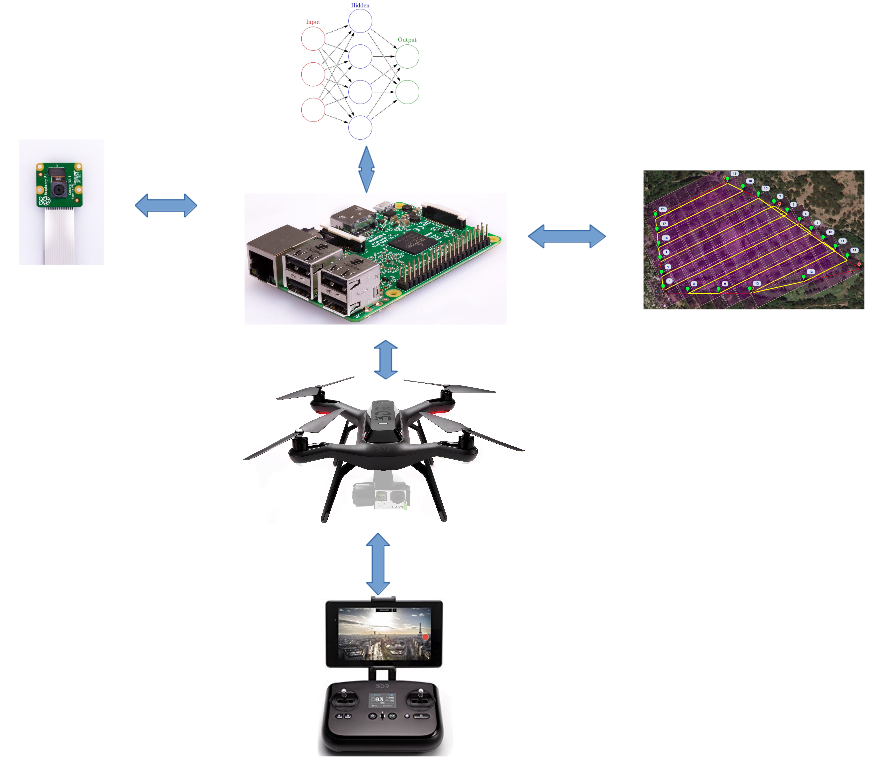
\includegraphics[width=.6\textwidth]{sistema}
	\caption{Esquema general del sistema propuesto}
	\label{Vista ventral}
\end{figure}


\section{Hipótesis}
A partir de los conocimientos previos, al implementar este sistema se pueden obtener buenos resultados ya que el sistema embebido nos proporciona la facilidad de integrar todos los elementos para la planificación, el procesamiento de la información y a su vez implementar una red neuronal sin colisionar con la memoria que integra el sistema embebido, sin embargo se puede esperar que el tiempo de respuesta para cada proceso puede ser una limitante para nuestro sistema ya que se requeriría un sistema embebido con capacidades de memoria y procesamiento que superen a las de una Raspberry Pi.

\section{Materiales}
Los siguientes materiales se utilizaran para el desarrollo del proyecto, esto puede variar en función del avance del trabajo.
\begin{itemize}
	\item Vehículo Aéreo no Tripulado (VANT) "3DR Solo".
	\item Raspberry Pi 3
	\item Cámara Raspberry NOIR
	\item Tableta electrónica
	
\end{itemize}

\section{Objetivo General}
Desarrollar un método de planificación de rutas para cubrir una superficie.
\section{Objetivos Específicos}
\begin{itemize}
	\item Realizar un estudio de diferentes técnicas de planificación de rutas y seleccionar el mas adecuado.
	\item Implementar mediante un sistema embebido  el desarrollo de un método para la planificación de la ruta adecuada del VANT.
	\item Desarrollar un método de planificación de áreas, utilizando técnicas o modelos matemáticos para la planeación el recorrido del VANT.
	
\end{itemize}


\chapter{Fundamento Teórico}
\section{Vehículo aéreo no tripulado (VANT)}

Un vehículo aéreo no tripulado (VANT) o (UAV) por su sigla en inglés es un aeronave que no requiere de la tripulación de un piloto a bordo.
Hay una gran diversidad de vehículos aéreos no tripulados, en este sentido se pueden diferenciar los móviles aéreos en tres grandes categorías.
\begin{itemize}
	\item VANT de ala fija, Son los vehículos que las alas se encuentran unidas por el resto de la aeronave, Estas aeronaves generan la sustentación básicamente por los planos, cuyo perfil aerodinámico está diseñado específicamente para crear diferencia de presión entre el intradós (parte inferior) y el extradós (parte superior).
	\item Multirrotores: Un multirrotor es una aeronave de ala rotatoria que posee tres o más rotores. Dependiendo del número de rotores y de su configuración, los multirrotores pueden subdividirse en diferentes tipos, yendo desde aeronaves con tres rotores (tricópteros o trirrotores), cuatro rotores (quadcópteros o cuatrirrotores) hasta configuraciones de 8 (octocópteros) o más rotores.
	\item VANT híbrido,Este tipo de RPAs son capaces de despegar y aterrizar de forma vertical, como las aeronaves de ala rotatoria, y de realizar vuelos a alta velocidad, como un ala fija tradicional.
	
	Estas aeronaves poseen redundancia de mecanismos de sustentación, lo que convierte a esta solución en una opción robusta ante fallos inesperados. Sin embargo, su estructura mecánica y de control es compleja. Fruto de esta complejidad, actualmente existen muy pocas ofertas comerciales de este tipo de drones, y las aeronaves que ya se encuentran en el mercado poseen precios sumamente elevados.
	
\end{itemize}
%\begin{figure}
%	\centering
%	\begin{minipage}{.45\textwidth}
%		\centering
%		\includegraphics[width=.5\linewidth]{PIX}
%		\caption{PIXHAWK}
%	\end{minipage}
%	\begin{minipage}{.45\textwidth}
%		\centering
%		\includegraphics[width=.5\linewidth]{dron}
%		\caption{Dron utlizado}
%	\end{minipage}
%\end{figure} 

La navegación de un vehículo aéreo no tripulado (VANT) requiere de diferentes marcos de referencia para poder especificar la posición del vehículo Estos marcos de referencias son necesarios para localizarse con respecto de la tierra o para planificar los caminos utilizando técnicas basadas en geometría euclidiana.\cite{garcia}\\

\section{Sistema embebido}
Un sistema embebido son sistemas hardware/software diseñados para un proposito especifico, diseñado para realizar una o mas tareas. Algunas de las características importantes en relación a las computadoras tradicionales son:
\begin{itemize}
	\item El costo de producción es bajo
	\item Se pueden implementar en diferentes arquitecturas de procesadores.
	\item Su desarrollo implica un diseño particular de hardware y software, con el objetivo de satisfacer la tarea especifica que se desea cumplir.
	\item En los sistemas embebido el consumo de potencia es un aspecto muy importante, porque permiten implementar soluciones con bajos consumos de energia.\cite{jimenez2011}
Particularmente para este trabajo se usó un sistema embebido Raspberry Pi 3b, lo cual dada sus características 

\end{itemize}

\section{Cobertura de área}
La cobertura de área es el proceso a seguir para encontrar un camino que cubra un área de interés, el cual este problema ha sido abordada por diferentes autores desde un punto de vista geométrico hasta cuestiones como el uso de energía del VANT, rapidez, aceleración y el procesamiento de imágenes. \cite{DiFranco}

\section{Redes neuronales convolucionadas}
Las redes neuronales son similares a las redes neuronales ordinarias, están formadas por neuronas que tienen sesgos y pesos que pueden aprender.  Toda la red todavía expresa una única función de puntuación diferenciable: desde los píxeles de la imagen sin formato en un extremo hasta los puntajes de clase en el otro. Y todavía tienen una función de pérdida (por ejemplo, SVM / Softmax) en la última capa (totalmente conectada) y todos los conceptos que se usan en las redes neuronales regulares todavía se aplican.\\
Lo que cambia en las arquitecturas ConvNet es que suponen explícitamente que las entradas son imágenes, lo que nos permite codificar ciertas propiedades en la arquitectura. Estos hacen que la función de reenvío sea más eficiente de implementar y reducen enormemente la cantidad de parámetros en la red.\\
Alguna de las características son las siguientes:\cite{ASH:2013:Online}
\begin{itemize}
	\item Cada capa oculta está formada por un conjunto de neuronas, donde cada neurona está completamente conectada a todas las neuronas en la capa anterior, y donde las neuronas en una sola capa funcionan de manera completamente independiente y no comparten ninguna conexión.
	\item . En CIFAR-10, las imágenes son solo de tamaño 32x32x3 (32 de ancho, 32 de alto, 3 canales de color), por lo que una sola neurona totalmente conectada en una primera capa oculta de una red neuronal normal tendría 32 * 32 * 3 = 3072 pesos.
	\item Las capas de una ConvNet tienen neuronas dispuestas en 3 dimensiones: ancho, alto, profundidad. 
\end{itemize}


\section{Robotic Operating Systems (ROS)}
\textbf{ROS} por sus ingles Robotic Operating Systems es un sistema flexible que permite escribir programas para robots. Es una colección de herramientas, bibliotecas y convenciones que tienen como objetivo simplificar  la tarea de crear un comportamiento de robot complejo y robusto en una amplia variedad de plataformas robóticas.\\
Desde la perspectiva del robot, los problemas que parecen triviales para los humanos a menudo varían enormemente entre instancias de tareas y entornos. Lidiar con estas variaciones es tan difícil que ningún individuo, laboratorio o institución puede esperar hacerlo solo.\\
\textbf{Herramientas} Una de las características importantes de ROS es el conjunto de herramientas de desarrollo. Estas herramientas permiten admiten la introspección, la depuración, el trazado y la visualización del sistema que se está desarrollando. ROS se puede usar sin usar una GUI. También nos permiten herramientas de manera gráfica como rviz y rqt.
\textbf{Rviz} nos proporciona visualización tridimensional de varios tipos de datos de sensores y cualquier robot descrito por URDF. Rviz puede visualizar muchos de los mensajes comunes proporcionados por ROS, como escaneo láser, nubes de puntos tridimensionales e imágenes de cámaras.
\textbf{Rqt} proporciona el desarrollo de interfaces gráficas para el robot. Se pueden crear interfaces personalizadas al configurar la extensa biblioteca de de plugins de rqt incorporado en pestañas, pantallas divididas y otros diseños.


%--------------------------------------------------------------------------
  
\chapter{Trabajo Relacionado}

\section{Planificación de rutas para cobertura de polígonos convexos}



Por otro lado también se ha realizado planificación con vehículos sub-acuáticos, el principio de funcionamiento es similar a la de un VANT, en este sentido Juan David Hernández propone un método de planificación para cubrir áreas en donde se hacen dos recorridos, el cual en el primer recorrido deja una brecha sin explorar, cubriéndolo así en el segundo recorrido, utilizando estrategias de planificación de re-planificación de rutas y cobertura de áreas. \cite{hernandez2017}\\

En la tesis de Gerardo Hernández propuso implementar un conjunto de técnicas para identificar objetos mediante VANT's en tareas de vigilancia, en donde se hace uso de la técnica "puntos de interés" que permiten extraer rasgos descriptores en donde las muestras contiene ruido, y a su vez presenta un software que permite visualizar las redes neuronales analizadas y presentar los resultados de clasificación en tiempo real de forma gráfica al usuario. \cite{hernandez2016}

Gramajo, et al. Presenta una estrategia de planificación de rutas para una misión de búsqueda y cobertura de un VANT, en donde maximiza el área cubierta, dadas las restricciones de operación y de energía la propuesta formula una gran autonomía para el vehículo sin requerir una selección exacta de parámetros de optimización.\\
La trayectoria que se plantea maximiza la ruta de vuelo y a su vez reduce el tiempo de vuelo, la comparación se realiza con algoritmos de planificación teniendo resultados similares, pero a su vez mejoran el rendimiento y posición inicial del vehículo.\cite{gramajo2017}\\

 \begin{figure}[!h]
 	\centering
 	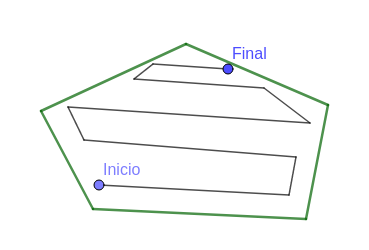
\includegraphics[width=.4\textwidth]{path_1}
 	\caption{Ejemplo de cobertura de área para un polígono convexo siendo inicio el despegue y final el aterrizaje}
 	\label{Path optima}
 \end{figure}

\section{Planificación de rutas para la cobertura de polígonos no convexos}

Un interesante ejemplo es la reconstrucción de un terreno  3D a partir de una imagen 2D tomadas de desde un VANT.
La propuesta de Marina Torres et al, para polígonos no convexos  se propone descomponer en un conjunto de múltiples polígonos convexos. Cuando se trata de polígonos no convexos el procedimiento para calcular la linea de vuelo óptimo es parecido al algoritmo para calcular la cobertura de un solo polígono convexo. Para este caso se descartan algunos aristas siguiendo el siguiente procedimiento:

\cite{torres2016}
\begin{figure}[!h]
	\centering
	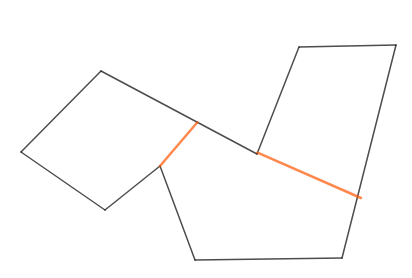
\includegraphics[width=.4\textwidth]{no_convex_polygon}
	\caption{Ejemplo de descomposición de un polígono no convexo}
	\label{descomposition_polygon}
\end{figure}

\subsection{Algoritmos para cobertura óptima de polígonos no convexos}
En el trabajo de Milán Rollo describe diferentes algoritmos para resolver el problema de cobertura de ruta para polígonos no convexos \cite{pereira2014}
\subsection{Planificador consciente del consumo de energía del VANT}

\subsection{Separación de partes cóncavas}

\subsection{Problema de múltiples rutas}


Las tres principales contribuciones de la tesis de Bochkarev se dan de la siguiente manera:
\begin{itemize}
	\item Se propone un método que calcula la altitud mínima de un polígono no convexo.
	\item Dada una descomposición convexa inicial de un polígono, se propone un método para reoptimizar iterativamente y eliminar los cortes de la descomposición para optimizar la altitud del polígono en cada lado del corte  
	\item En tercer lugar, calculan una ruta de cobertura del área de trabajo colocando segmentos de línea paralelos en cada región, y luego calculando un recorrido de longitud mínima de la descomposición convexa aproximada correspondiente
\end{itemize} \cite{bochkarev2017}



\section {Vuelos autónomos}
João Pedro Carvalho, et al. Propuso un sistema de interacción entre el usuario y el VANT para vuelos autónomos, donde el cálculo necesario se realiza en una sistema embebido incorporado, disminuyendo el tiempo de respuesta y eliminando la necesidad de realizar enlaces a larga distancia a una estación de tierra. Los resultados se presentan con el hardware en las simulaciones de bucle, también se presenta un VANT que usa Pixhawk, odroid y ROS como plataforma complementaria de computadora y software para el desarrollo de código.\\
La aplicación propuesta en este trabajo utiliza un quadrotor comercial IRIS para lograr una misión totalmente autónoma sin depender de bases terrestres. Por lo tanto, una computadora (Odroid) está incrustada en el avión para calcular sus comandos de control durante la misión.
 Este trabajo muestra una plataforma embebida con alto poder computacional para el desarrollo de navegación autónoma de vehículos aéreos no tripulados con procesamiento de datos  en tiempo real, como la visión por computadora, sin depender del enlace de comunicación de la estación terrestre. \cite{carvalho2017s}
 \begin{figure}[!h]
 	\centering
 	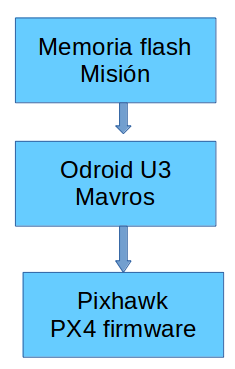
\includegraphics[width=.4\textwidth]{connection}
 	\caption{Conexión del hawrdare}
 	\label{hw connection}
 \end{figure}
 
 
\subsection{Redes neuronales en sistemas embebidos}
En el trabajo de Clement Farabet, et al. Se presenta una arquitectura hardware para implementar una red neuronal convolucional en un FPGA y ASIC que muestra la rapidez de ejecución, el modelo de la FPGA es Xilinx Virtex-4 SX35 el cual se conectó un una memoria RAM en donde el objetivo es detección en tiempo real, reconocimiento y segmentación de imágenes de megapixeles, dentro de la arquitectura, los componentes que destacan son: una unidad de control, ALU's paralelos múltiples, transmisión de interfaz de memoria.\\
%------------------------------------------------------------
\chapter{Planificación de la ruta de cobertura con VANTs}
Esta tesis está centrada en el planificador \cite
Para que una planificación de ruta se pueda realizar se requieren se consideran los siguientes puntos.
\begin{itemize}
	\item Traslape de fotografías:
	\item Orientación
\end{itemize}

\section{Marcos de referencia}
Los marcos de referencia se usan para localizar un objeto en el plano o en espacio, los sistemas de navegación requieren de la medición y cálculos entre marcos de referencia.


\subsection{Sistema de coordenada geodésico}
El sistema de coordenada geodésico es ampliamente usado para sistemas de navegación basadas en GPS ya que es un sistema que caracteriza una coordenada cerca a la superficie de la tierra en términos de latitud ($\lambda$), longitud ($\phi$) y altura ($h$).\\
La latitud mide el ángulo (de -90$^{\circ}$ a 90 $^{\circ}$) entre el plano ecuatorial y el normal  de la elipsoide de referencia que pasa mediante el punto medido. La longitud mide el ángulo rotacional (de -180$^{\circ}$ a 180$^{\circ}$) entre el primer meridiano y el punto medido.\\
Los parámetros importantes en coordenadas geodésicas incluye:
\begin{itemize}
	\item Semieje mayor $R_{Ea}$
	\item Factor de aplanamiento $f$
	\item Semieje menor $R_{Eb}$
	\item Primera excentricidad $e$
	\item Radio del meridiano de la curvatura $M_{E}$
	\item Primer radio vertical de la curvatura $N_{E}$
\end{itemize}
En donde:
\begin{equation}
	R_{Ea} = 6,378,137.0 m,
\end{equation}
\begin{equation}
	f = 1/298.257223563,
\end{equation}
\begin{equation}
R_{Eb} = R_{Ea} (1-f)  = 6,356,752 m,
\end{equation}
\begin{equation}
e = \frac{\sqrt{R_{Ea}^{2}-R_{Eb}^{2}}}{R_{Ea}}= 0.08181919, \label{4:1}
\end{equation}
\begin{equation}
R_{Eb} = \frac{R_{Ea}(1-e^{2})}{(1-e^{2}\sin^{2}\phi)^{\frac{3}{2}}}
\end{equation}
\begin{equation}
N_{E}=\frac{R_{Ea}}{\sqrt{1-e^{2}\sin\phi}} \label{4:6}
\end{equation}

\subsection{Sistema de coordenada Earth-Centered Earth-Fixed ECEF}
Esta coordenada tiene su origen en el centro fijo de la tierra, tiene su exe x extendido mediante la intersección del primer meridiano (0$^{\circ}$ Longitud) y el ecuador (0$^{\circ}$ Latitud). El eje z se extiende mediante el polo norte verdadero.

\subsection{Sistema de coordenadas NED (North East Down)}
El sistema de coordenadas local NED su origen y sus ejes están definidos por los siguientes elementos:
\begin{itemize}
	\item El origen (denotado por $O_{n}$) es arbitrariamente fijado a un punto en la superficie de la tierra
	\item El eje X (denotado por $X_{n}$) apunta hacia el elipsoide norte (norte geodésico)
	\item  El eje Y (denotado por $Y_{n}$) apunta hacia el elipsoide este (este geodésico)
	\item El eje Z (denotado por $Z_{n}$) apunta hacia abajo a lo largo del elipsoide normal
\end{itemize}
El marco de referencia NED juega un papel importante en el control de vuelo y navegación de VANTs de pequeña escala.

\section{Transformación de coordenadas}
\subsection{Sistema de coordenadas geodesico y ECEF}
La transformación de la posición del vector del sistema geodesico a coordenadas ECEF es un paso intermedio para la medición de la posición GPS al sistema de coordenadas NED. Dado un punto en el sistema geodesico decimos que:
\begin{equation}
P_g = \begin{pmatrix} \lambda \\ \phi \\ h  \end{pmatrix}
\end{equation}
Sus coordenadas en el marco ECEF está dado por:
\begin{equation}
P_e = \begin{pmatrix} \lambda \\ \phi \\ h  \end{pmatrix} = \left[ \begin{array}{c} (N_E + h) \cos\phi\cos\lambda \\ (N_E + h) \cos\phi \sin\lambda \\ (N_E(1- e^2) + h) \sin \phi \end{array} \right]
\end{equation}
Donde $e$ y $N_E$ estan dados por \ref{4:1} y \ref{4:6} respectivamente.

\subsection{Sistemas de coordenadas ECEF y el local NED}
La transformación del marco de referencia ECEF al marco local NED se requiere la transformación del sistema geodésico al ECEF y viceversa en conjunto.
En donde se tiene:
\begin{equation}
P_n = R_{n/e} (P_e - P_{e,ref})
\end{equation}

Donde $P_e,ref$ es la posición del origen del marco local NED (normalmente el punto de despegue del VANT) en el sistema de coordenadas ECEF y $R_n/e$ es la matriz de rotación del marco de referencia ECEF al sistema local NED, que está dado por:

\begin{equation}
A = \begin{bmatrix}
-\sin\phi_{ref} \cos\lambda_{ref} & -\sin\phi_{ref} \sin\lambda_{ref} & \cos\phi_{ref} \\
-\sin \lambda_{ref} & \cos \lambda_{ref} &  0 \\
-\cos\phi_{ref} \cos\phi_{ref} & -\cos\phi_{ref} \sin\lambda_{ref} & -\sin\phi_{ref}
\end{bmatrix}
\end{equation}

Donde $\lambda_{ref}$ y $\phi_{ref}$  son latitud y longitud respectivamente de $P_{e,ref}$


\section {Planificación de cobertura de ruta óptima basado en el algoritmo \textit{rotating calipers}}
El campo de aplicación mediante VANTs ha sido exitoso en actividades como aplicación de mapeo, agricultura de precisión, vigilancia, entre otros. Actualmente uno de los problemas a resolver es planificar una ruta para el VANT cuando la ruta es implementada en un terreno y a su vez escanearlo. tal problema es conocido como planificación de cobertura mediante rutas.
Se propone un método eficiente con complejidad O(n), al calcular la cobertura óptima de la ruta para un área. La optimización está definida en términos de tiempo que el VANT necesita para seguir la ruta. El método esta basado en el calculo de puntos antipodales propuesto por Shamos \cite{shamos1978} el cual se asemeja a un calibrador que mide el tamaño de un polígono. El algoritmo propuesto es una pieza fundamental en tareas mas complejas como vigilancia en áreas disjuntas o inspección de fachadas de edificio, donde cada cara del edificio representa un polígono.

\begin{figure}[!h]
	\centering
	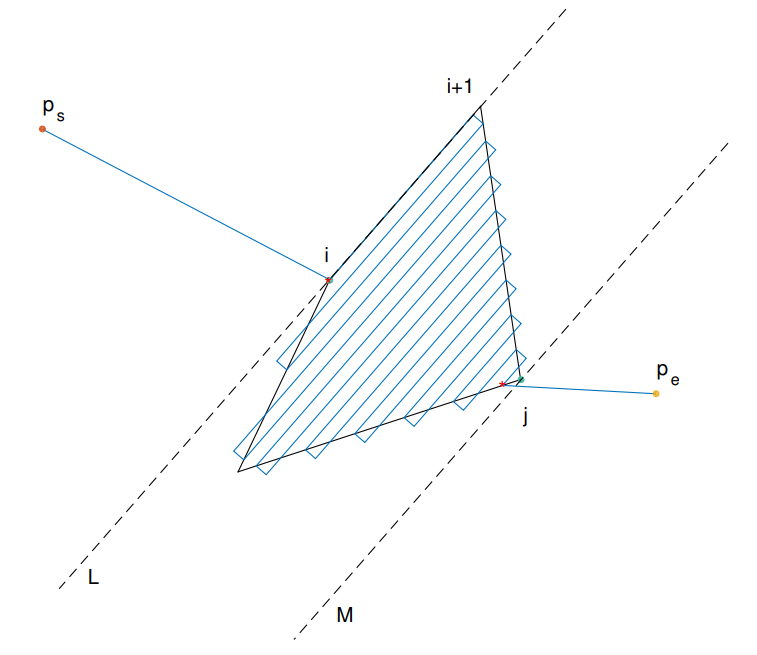
\includegraphics[width=.4\textwidth]{caliper}
	\caption{Ejemplo de una cobertura óptima de ruta. En donde la ruta (lineas azules) inicia con el despegue del VANT $\rho_s$, sigue un patrón de ida y vuelta dentro del área a explorar (polígono en negro) y mueve al punto de aterrizaje $\rho_e$.}
	\label{fig:caliper}
\end{figure}

El problema está orientado a encontrar una ruta que cubra un área a explorar en un tiempo mínimo tomando en cuenta desde el punto de inicio al punto de aterrizaje.

\subsubsection{Suposiciones y definiciones}
Se asume que que el área a explorar es planar y está definida por un polígono convexo, $Q={V,E},$ Donde $V = {1,...,n}$ es un conjunto de vértices ordenadas en el sentido de las manecillas del reloj y $E = {(1,2),...,(n-1),(n,1)}$ es el conjunto de aristas. El VANT es un multirotor y asumimos que durante el vuelo sigue dos movimientos primitivos, de rotación y traslación en sitio. 
El VANT toma el punto de despegue $\rho_s$ y el de aterrizaje el punto $\rho_e$, ambos puntos pueden estar dentro o fuera del polígono. Cuando el VANT recorre un área, inicia en el punto inicial, vuela sobre el área, sigue un patrón de búsqueda y termina en el punto de aterrizaje.
Un patrón de búsqueda es una ruta que sigue el dron para cubrir un area. Se usa un patrón de idea y vuelta (PIV) donde el VANT sigue lineas rectas dentro del poligono. Las distancia entre las lineas de vuelo depende de la cámara y de la resolución espacial deseada. Una de las ventajas del patrón de ida y vuelta es que pueden ser resumidas en $\rho = \{p_0,...,p_m\}$.
Para cada waypoint de la ruta, el VANT se orienta por si mismo y se mueve en linea recta. Si se incluyen los puntos de despegue y aterrizaje, la ruta estaria dada por $\tau = \{ p_s, p_0,...,p_m, p_e\}$.

\begin{algorithm}[H]
	\SetAlgoLined
	 \KwData{$V, \rho_s, \rho_e$}
	\KwResult{$\tau$}
	A $\longleftarrow$ calculoParesAntipodales(V)\;
	$c^*$ $\longleftarrow$ $\infty$\;
	
	\ForEach{(i,j) $\in$ A}{%
		$\rho \gets MejorRuta(V,i,j)$\;
		\If{$costo(\{\rho_s, \rho, \rho_e\}) < c^*$}{%
			$\tau \gets \{\rho_s, \rho, \rho_e\}*$\;
			$c* \gets (\tau) $
		}
	}
	%\KwRet{$Q^*$}\;
\caption{Cobertura óptima de una ruta}
\end{algorithm}

\subsubsection{Método propuesto}
 El método propuesto por J. Irving et al. \cite{gomez2017}  
 Cuando un patrón de ida y vuelta es usado para cubrir un área cada linea de vuelo es paralelo de la siguiente, así que las lineas de vuelo inicial y final son paralelos. Ahora reemplazamos las lineas de vuelo de la PIV con lineas imaginarias de soporte $L$ y $M$. \ref*{fig:caliper}

Una linea de soporte puede pasar solo mediante un vértice o en la unión de un arista con el poligono. En el caso donde el vértice toca 
\chapter {Sistema embebido a bordo del VANT}

En el contexto de los sistemas embebidos se encuentra la tarjeta Raspberry Pi 3 que es un ordenador de placa reducida de bajo costo, gracias a las características que contiene se pueden realizar procesos computacionales para realizar determinada acción, en este sentido se usó para el procesamiento de imágenes a bordo del VANT, dotar de autonomía al VANT mediante redes neuronales y planificación de trayectorias para lo cual se requiere una tarjeta SD de al menos 2Gb, cámara Raspberry Pi, cable plano de 15 hilos para la cámara, cable HDMI para visualizar la interface gráfica y accesorios como ratón y teclado.\\
Para añadir la Raspberry al VANT se realizaron algunas modificaciones para asegurar su colocación de forma tal que tanto su peso como su posición no imposibilitara el despegue y el funcionamiento del VANT.
\begin{figure}[!h]
	\centering
	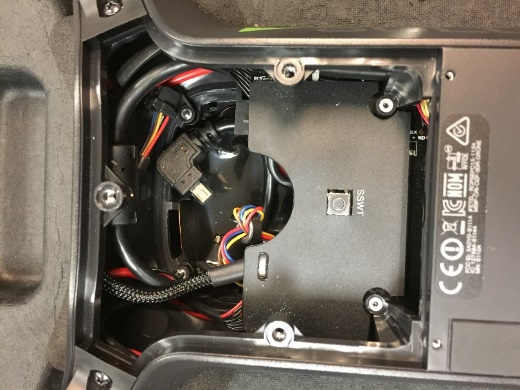
\includegraphics[width=.6\textwidth]{dos}
	\caption{Vista posterior ventral del VANT}
	\label{Vista ven}
\end{figure}

\subsection{Acoplo de alimentación para la Raspberry Pi 3}

Se añadió un cable de alimentación tipo micro USB y un switch (on/off) al portapilas que alimenta a la Raspberry para controlar el encendido y apagado del embebido.
\begin{figure}[!h]
	\centering
	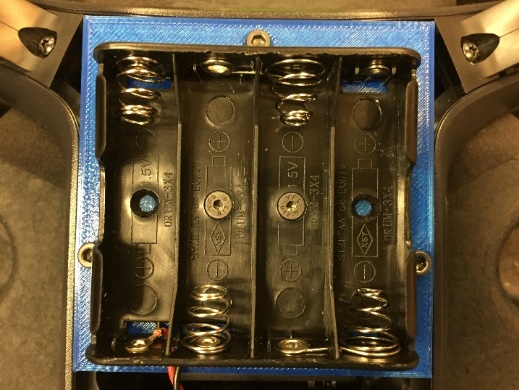
\includegraphics[width=0.6\textwidth]{cinco}
	\caption{Porta pilas sujeto al VANT a través de la base}
	\label{Anclaje total}
\end{figure}

Una vez resuelto el tema de la alimentación de la Raspberry Pi, se procedió a identificar el modo de añadir dicho sistema embebido, minimizando la posibilidad de desestabilizar al VANT para una cámara. El diseño de la figura 6 se obtuvo del sitio  \url{http://www.thingiverse.com/thing:1474960/#files}, bajo la licencia de Creative Commons,ademas de basarnos en el plano del VANT en donde especifica el tamaño y la posición exacta de los tornillos,en donde a su vez contiene los orificios necesarios para adherir los tornillos a la placa en donde se sujetó al VANT de la parte ventral anterior, utilizando los orificios que el propio VANT ya tenia para la sujeción de accesorios secundarios.
\begin{figure}[!h]
	\centering
	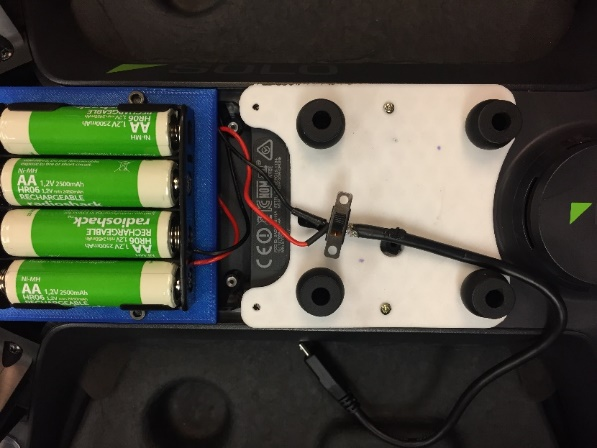
\includegraphics[width=0.6\textwidth]{ocho}
	\caption{Base de adaptación sujeta al VANT}
	\label{Base de Vant y pila}
\end{figure}

\subsection{Acoplamiento completo de la Raspberry y baterias al VANT}
Una vez adherida la placa al VANT tambien se adhirió unos soportes de goma para sujetar la siguiente placa y a su vez estabilizar la cámara de la Raspberry
\begin{figure}[!h]
	\centering
	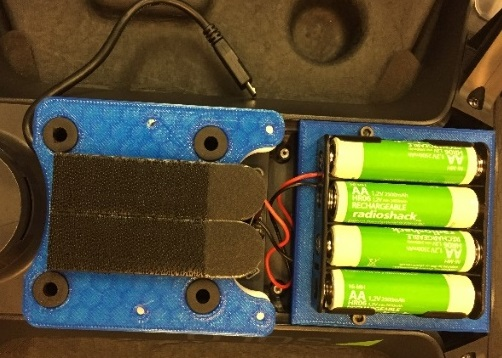
\includegraphics[width=0.6\textwidth]{diez}
	\caption{Bases de adaptación sujetas al VANT}
	\label{adaptacion completa}
\end{figure}

En la siguiente figura se muestra el sistema embebido con la cámara y su alimentación en el VANT siendo la vista final del acoplamiento del sistema embebido y su alimentación.
\begin{figure}[!h]
	\centering
	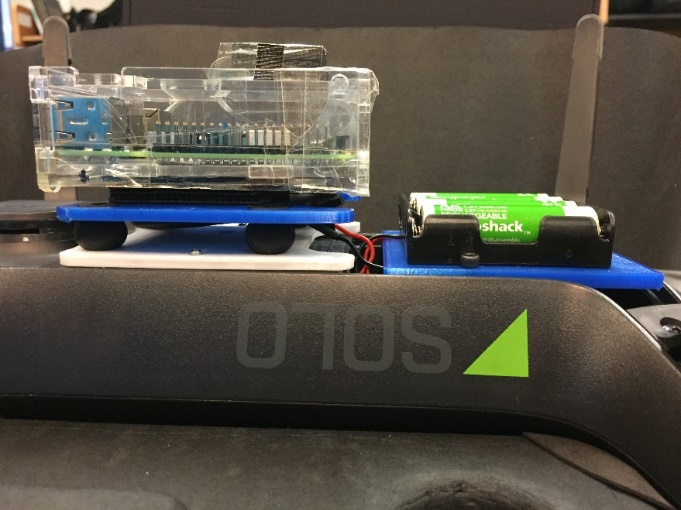
\includegraphics[width=0.6\textwidth]{doce}
	\caption{Raspberry montada al VANT 3DR Solo}
	\label{vista frontal}
\end{figure}
Para verificar su estabilidad y el funcionamiento del VANT se realizaron diferentes pruebas, descartando cualquier averia durante el vuelo.
\begin{figure}[!h]
	\centering
	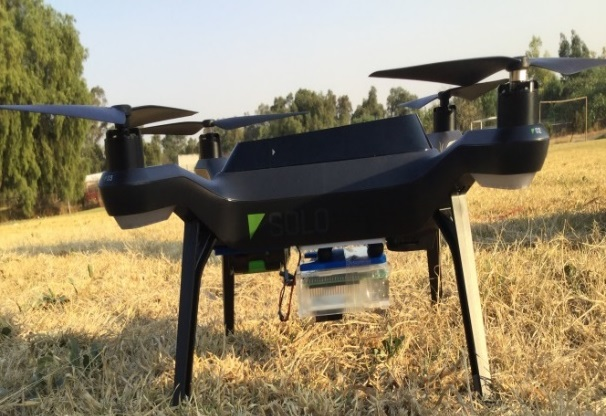
\includegraphics[width=0.6\textwidth]{catorce}
	\caption{Puesta en marcha del VANT}
	\label{VANT final}
\end{figure}

\section{Procesamiento de imágenes en la Raspberry Pi 3 con OpenCV}

\chapter{Reconocimiento de cactus con redes neuronales}


\chapter{Conclusiones}
 

%---------------------------------------
%Bibliografia
\bibliographystyle{plain}
\bibliography{bibliography}



\end{document}          
